%%%%%%%%%%%%%%%%%%%%%%%%%%%%%%%%%%%%%%%%%
% a0poster Portrait Poster
% LaTeX Template
% Version 1.0 (22/06/13)
%
% The a0poster class was created by:
% Gerlinde Kettl and Matthias Weiser (tex@kettl.de)
% 
% This template has been downloaded from:
% http://www.LaTeXTemplates.com
%
% License:
% CC BY-NC-SA 3.0 (http://creativecommons.org/licenses/by-nc-sa/3.0/)
%
%%%%%%%%%%%%%%%%%%%%%%%%%%%%%%%%%%%%%%%%%

%----------------------------------------------------------------------------------------
%	PACKAGES AND OTHER DOCUMENT CONFIGURATIONS
%----------------------------------------------------------------------------------------

\documentclass[a0,portrait]{a0poster}

\usepackage{multicol} % This is so we can have multiple columns of text side-by-side
\columnsep=100pt % This is the amount of white space between the columns in the poster
\columnseprule=3pt % This is the thickness of the black line between the columns in the poster

\usepackage[svgnames]{xcolor} % Specify colors by their 'svgnames', for a full list of all colors available see here: http://www.latextemplates.com/svgnames-colors

\usepackage{times} % Use the times font
%\usepackage{palatino} % Uncomment to use the Palatino font

\usepackage{graphicx} % Required for including images
\graphicspath{{figures/}} % Location of the graphics files
\usepackage{booktabs} % Top and bottom rules for table
\usepackage[font=small,labelfont=bf]{caption} % Required for specifying captions to tables and figures
\usepackage{amsfonts, amsmath, amsthm, amssymb} % For math fonts, symbols and environments
\usepackage{wrapfig} % Allows wrapping text around tables and figures
\usepackage[utf8]{inputenc}
\usepackage{cite}

\begin{document}

%----------------------------------------------------------------------------------------
%	POSTER HEADER 
%----------------------------------------------------------------------------------------

% The header is divided into two boxes:
% The first is 75% wide and houses the title, subtitle, names, university/organization and contact information
% The second is 25% wide and houses a logo for your university/organization or a photo of you
% The widths of these boxes can be easily edited to accommodate your content as you see fit

\begin{minipage}[b]{0.75\linewidth}
\veryHuge \color{NavyBlue} \textbf{Proposta de um Modelo para Comportamentos Não-Normativos} \color{Black}\\ % Title
\huge Ontologia e Sistemas MultiAgentes\\[0.4cm] % University/organization 
\end{minipage}

\begin{center}
	
\includegraphics[width=0.1\linewidth]{logoone}
	
\includegraphics[width=0.05\linewidth]{logocopel}
	
\includegraphics[width=0.05\linewidth]{onereal}
\end{center}
%
\vspace{1cm} % A bit of extra whitespace between the header and poster content

%----------------------------------------------------------------------------------------

\begin{center}\vspace{1cm} 
		\label{figUmlModelSimulation}
		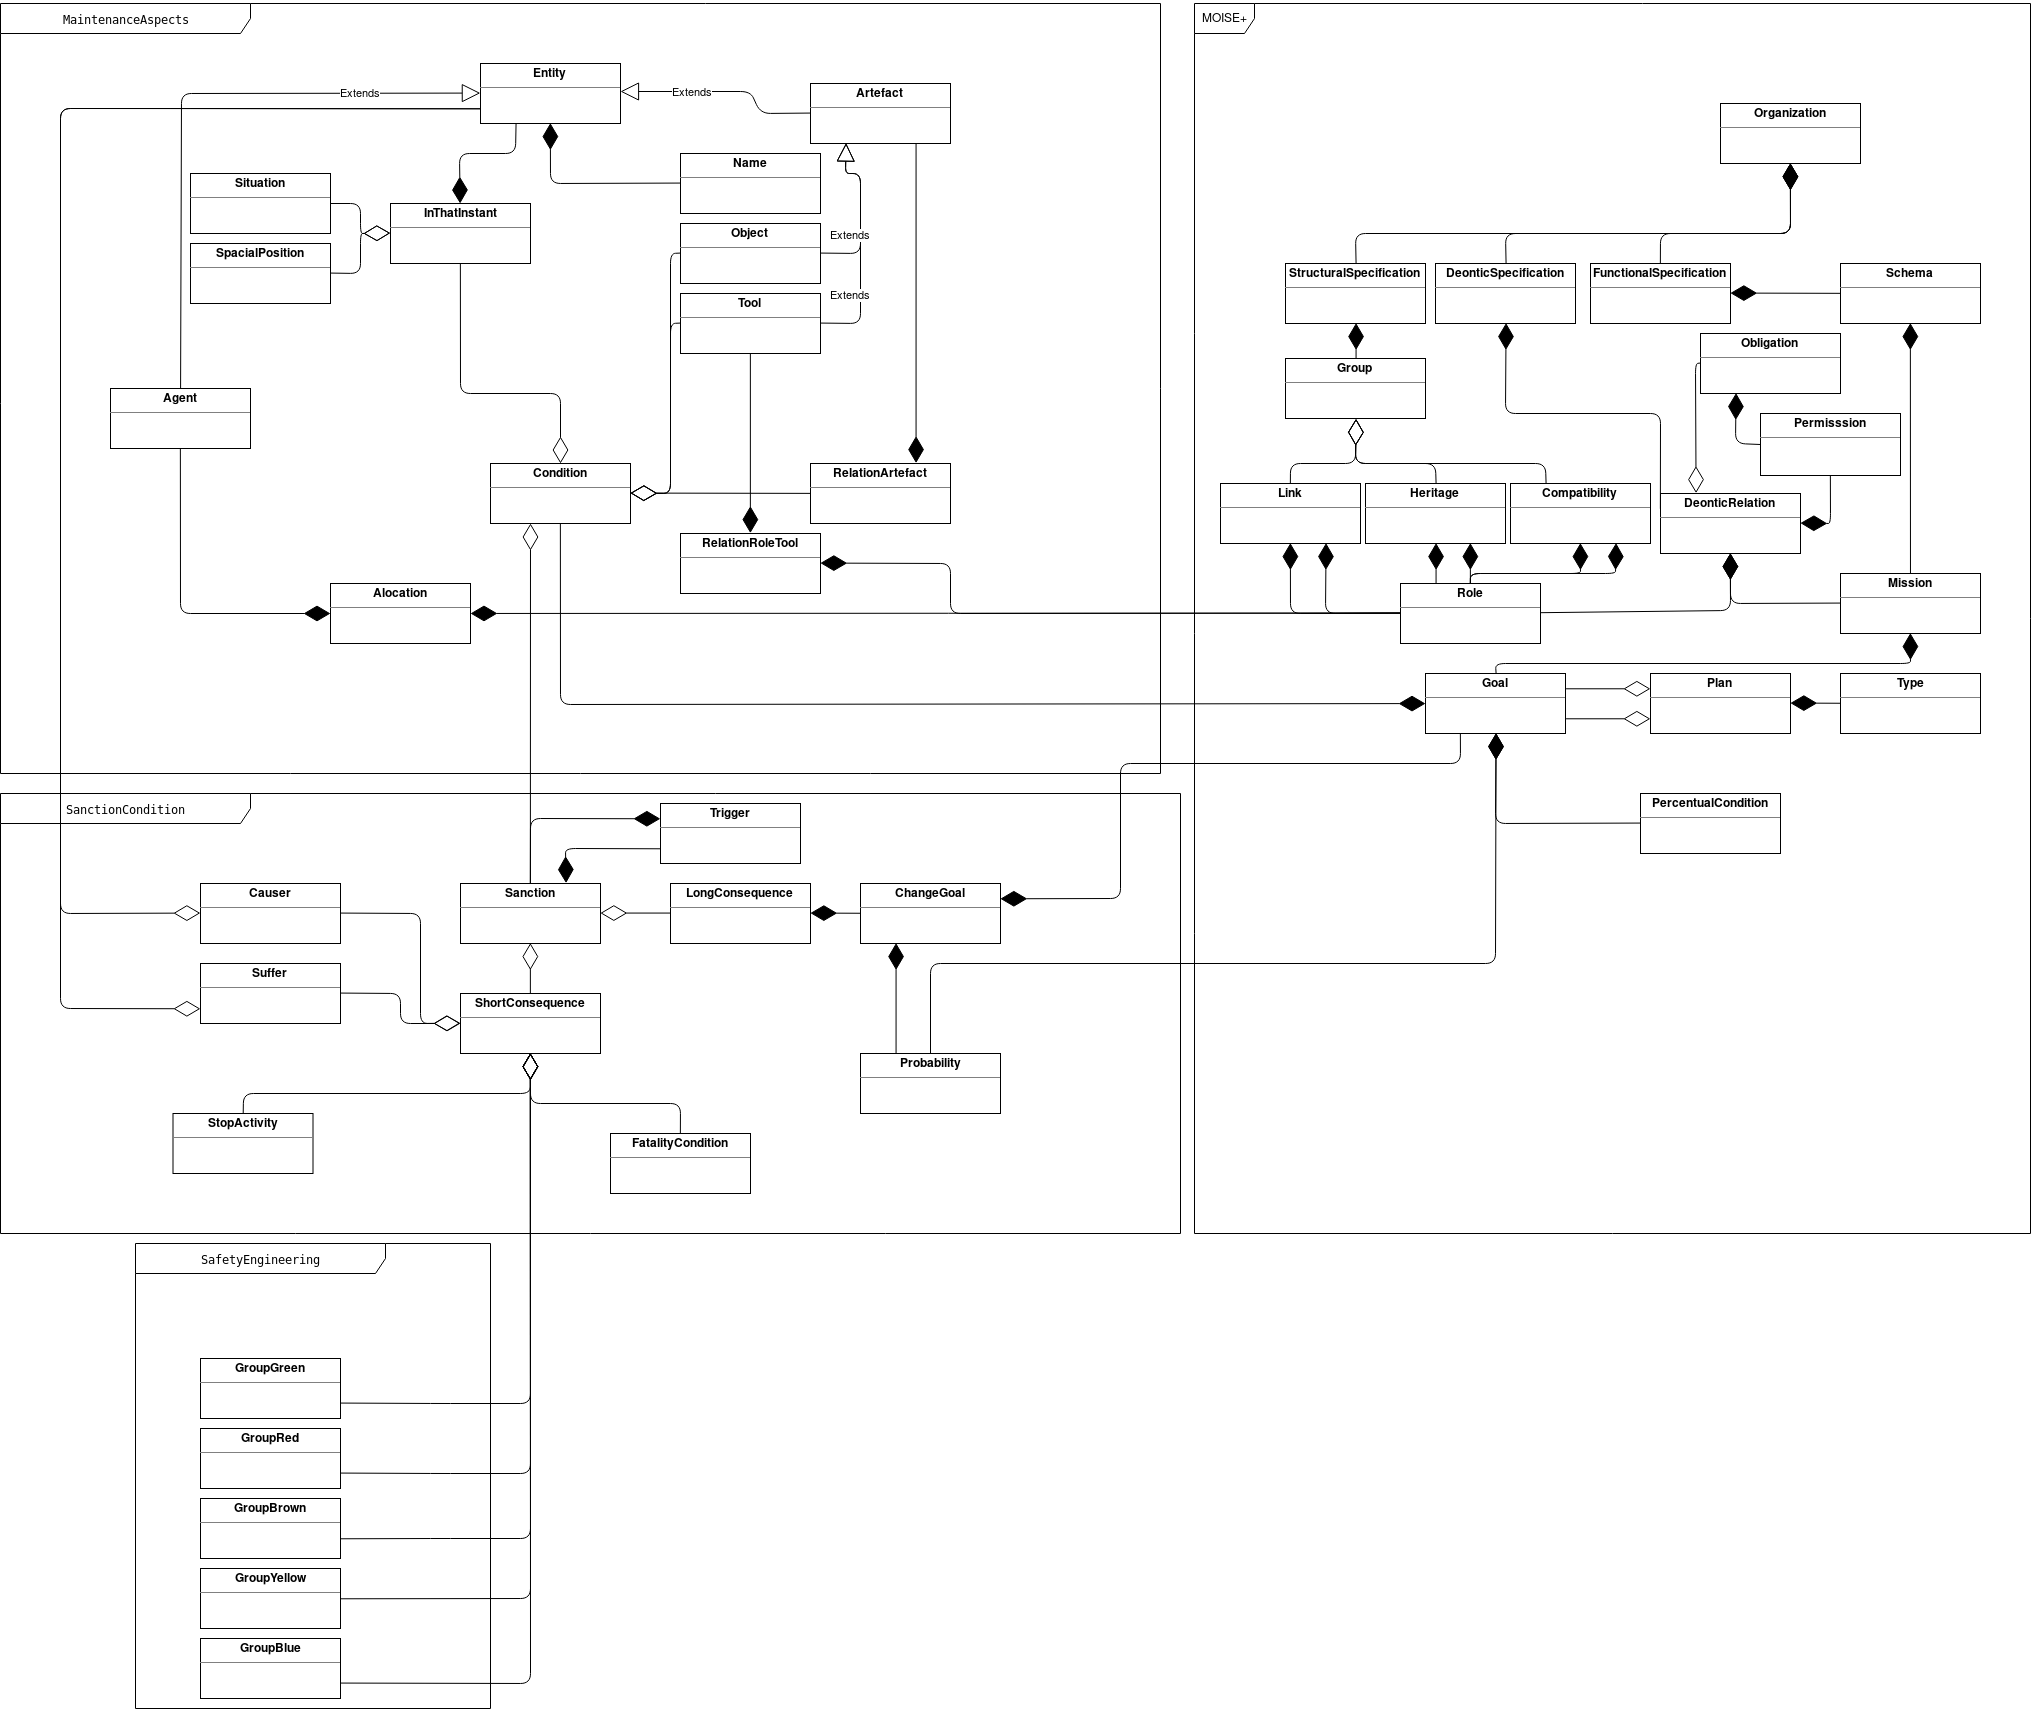
\includegraphics[width=0.65\linewidth]{uml_model_simulation}
		\captionof{figure}{\color{Green} Modelo resultante deste estudo escrito em UML}
\end{center}\vspace{1cm} 


\begin{multicols}{2} % This is how many columns your poster will be broken into, a portrait poster is generally split into 2 columns

\color{Navy} % Navy color for the abstract


%----------------------------------------------------------------------------------------
%	INTRODUCTION
%----------------------------------------------------------------------------------------

\color{SaddleBrown} % SaddleBrown color for the introduction


\color{} % DarkSlateGray color for the rest of the content


\section*{Descrição}

A primeira etapa metodológica desta pesquisa consistiu em identificar modelos que podem ser
usados para a finalidade deste estudo. Os pesquisadores identificaram um modelo em específico 
denominado de MOISE+\cite{AutonomousAgent}. O MOISE visa especificar o comportamento de um 
\textit{MAS} - Sociedade Multi-Agente. O MOISE+ leva em consideração que cada agente deve ter
um papel. Esse papel está vinculado a uma determinada missão. Está, por sua vez, engloba 
uma série de objetivos. O MOISE+ também leva em consideração questões organizacionais envolvendo
grupos, links e compatibilidades entre papeis. Este modelo apresenta relações de obrigação,
contudo não define relações de violação para as obrigações. Para a tratativa de violação de uma
norma, foi feito uso dos conceitos presentes no estudo \cite{ControllingNonNormative}.

A segunda etapa metodológica desta pesquisa consistiu em analisar o caso de estudo (manutenção em linha viva).
Para isso os pesquisadores analisaram procedimentos de manutenção sendo postos em prática, analisaram 
documentos técnicos, entrevistaram engenheiros especialistas na área. 

A terceira etapa metodologia se deu por criar conceitos, criar relações, adaptar conceitos de outros modelos, 
definir relações dos conceitos novos com os conceitos de outros modelos e verificar como este modelo resultante
se adapta ao estudo de caso.

A quarta etapa metodológica consistiu usar todos o material desenvolvido na terceira etapa na criação 
de um UML.

A quinta etapa metodológica se deu por implementar o modelo em Prolog (linguagem de programação). Para isso
o modelo foi escrito em relacionamentos de predicados. Uma vez feito isso, os pesquisadores realizaram diversas
consultas e inferências a fim de identificar relações de interesse a pesquisa. 

A sexta etapa consistiu em verificar se o modelo estava de acordo com o esperada tanto em relação a realidade 
como em relação aos seus propósitos.

\section*{Resultados}

A figura 1 apresenta uma representação em UML do modelo resultante. A figura estrutura em 
quatro blocos principais. O bloco \textit{MaintenanceAspects} apresenta todos os aspectos vinculados a manutenção 
propriamente dita, o bloco \textit{SanctionCondition} apresenta as sanções que ocorrem na violação de uma norma, o 
bloco \textit{MOISE+} consiste em uma representação similar ao modelo \textit{MOISE+} e o bloco \textit{SafetyEngineering}
apresenta todos os possíveis riscos com base em critérios de engenharia de segurança.


Inspirado no \textit{MOISE+}, este modelo define uma relação deôntica de obrigatoriedade com base na missão e no papel. 
Contudo, também assume como verdade a seguinte relação. 

\begin{equation}\label{deontilogic}
	obligation(\rho,mission)\wedge hasGoal(mission,goal) \to obligation(\rho,goal)
\end{equation}

A relação na implacabilidade \ref{deontilogic} tem que ser assumida como verdadeira, pois uma sanção é especificada em 
relação ao objetivo propriamente dito. Outro relação importante é \label{sanction} em que a não execução de uma obrigação
implicação na ocorrência de uma sanção.
\begin{equation}\label{sanction}
		  \sim obligation(\rho,goal) \wedge hasSanctionName(name_{sanction}) \to sanction(\rho,goal,name_{sanction})
\end{equation}

A relação \ref{lconsequence} significa que uma sanção implica em consequências de longo prazo em um outro objetivo.
\begin{equation}\label{lconsequence}
		  sanction(\rho,goal,name_{sanction}) \wedge isInstanceOf(goal_{b},goalClass) \to longConsequence(goal_{b}) 
\end{equation}
A relação \ref{lconsequence1} define que uma consequência de longo prazo faz com que a probabilidade de um objetivo dar certo
mude.
\begin{eqnarray}\label{lconsequence1}
	longConsequence(goal) \wedge hasProbability(goal,probability) \wedge exist(newProbability) \nonumber \\ 
	\to hasProbability(goal,newProbability)
\end{eqnarray}
A relação \ref{lconsequence2} define que a nova probabilidade de um objetivo dar certo tem que ser necessariamente menor
do que a probabilidade antiga.
\begin{equation}\label{lconsequence2}
	 hasProbability(goal,newProbability)\to (newProbability < probability)
\end{equation}


A relação \ref{risk} define que toda sanção apresenta consequências de curto prazo (no próprio objetivo). A consequência
implica na ocorrência de um risco associado a atividade, como no risco de ser eletrocutado. Pelo UML, é possível verificar
que o risco deve necessariamente pertencer aos possíveis riscos definidos por Engenharia de Segurança. O risco também 
é associado a um certo grau de fatalidade.
\begin{equation}\label{risk}
	sanction(\rho,goal,name_{sanction}) \to exist(risk,\rho) 
\end{equation}
A relação \ref{sanctionTrigger} define que a ocorrência de uma sanção dispara outra sanção.
\begin{equation}\label{sanctionTrigger}
	trigger(name_{sanction-start},name_{sanction-fire}) \to happens(name_{sanction-start})
\end{equation}
A relação \ref{sanctionTrigger02} define que uma sanção pode ocorrer por algum motivo, como esquecer ferramenta certa para determinado objetivo.
\begin{equation}\label{sanctionTrigger02}
	trigger(name_{sanction-start},reason) \to happens(name_{sanction-start})
\end{equation}


----------------------------------------------------------------------------------------
\bibliographystyle{plain} % Plain referencing style
\bibliography{sample} % Use the example bibliography file sample.bib

\end{multicols}
\end{document}
